

\documentclass[12pt,a4paper]{report}
\usepackage{url,color}
\usepackage[portrait]{geometry}
\usepackage{graphicx}
\usepackage{tikz-er2}
\usepackage{graphicx}

\title{Employability Skills Development Laboratory \\ \Large Interior Designing Interface And Management System.}

\author{ Saurabh Bahulikar\and Tushar Dahibhate \and Sushant Dharmadhikari \and Suvrat Dharmadhikari \and Aishwarya Gajjal \ Soniya Gosavi\\\\  Project Guide: \\ Professor. P.M.Kamde \\\\ Computer Department, Sinhgad College of Engineering.}
\date{\today \\ First Created on August 07, 2014.} 

\pagenumbering{Roman}
\begin{document}
\maketitle
\begin{abstract}
This mini-project is the modeling scheme of an interior design and finance enterprise. It has been created in a two tier architecture database mechanism, wherein the database is generated using the MySQL server and the User Interface used to access this data is generated using NetBeans platform. The two tier functionality of accessing and fetching the data from the database to the UI on request of the user is carried out by a Java Data Base Connector (JDBC). The parameters used like the entities and relations between the various elements of the database are represented further using Entity-Relationship (E-R) diagrams. Lastly, the various test cases and the coding part required for it is put forth.
\end{abstract}

\tableofcontents

\chapter{Introduction.}%Chapter1
\pagenumbering{arabic}
The employability skills development lab is a new initiative introduced by the University of Pune, under the Third Year course of Computer Engineering to emphasize and embed the necessary skills related to industrial training approach.

\section{Choice of topic}
The topic which our group has shortlisted is about interior designing and the finances associated with this business. The prerequisite of this course required us to create a database as a backend, and create a Graphical User Interface (GUI) design as the frontend. Further, we had to link the database to the User Interface using a database connection mechanism. The chosen topic provides a good moral to the creation of database, GUI and the linkage between the two.

\section{Why interior designing?}
In today's world the people who can afford the benefits of owning a permanent house tend to renovate the interiors to cope up with the lastest trend's of living. Interior Designing has emerged itself to be a promising industry and it also creates a perfect idea for a database project. The database used, can be referred as a model, reflecting the various occupations and jobs created under the interior designing industry. The corporate infrastructure in our database is hierarchical in nature, originating with the owner and concluding with the workers. Therefore the topic was short-listed out of all possible topics. 

\section{About the application}
Interior Designing interface and management system is an application which is basically useful for both the customers and the administrators. This software has been developed for “Imperio Designers”. Administrators can manipulate the information which includes details regarding the departments and the workforce. The application will further allow customers to secure a guest login. Customers will be able to access the inventory and the details regarding the company. Cost estimation is also provided to the customers. 

\section{Objective}
The objective behind designing the Interior Designing Interface and Management System is to automate the traditional pen-paper approach and to make everything available at the click of a button. Also the information about the workforce and inventory can be maintained with ease.

\section{Scope}
Scope is the system on which the software can be installed. The project is developed to work as an desktop application. It can later be modified to operate over the internet.
%END OF CHAPTER1.

\chapter{System Analysis}%Chapter2

\section{Introduction}
Analysis can be defined as breaking up of any whole so as to find out their nature, function etc. It defines design as to make preliminary sketches, pattern or outline for the plan. System analysis and design can be characterized as a set of techniques and processes, a community of interests, a culture and an intellectual orientation.

\section{Existing System}
The Existing system is a brochure for the customers. Here the cost estimation will be carried out in the hand written registers. Also the Employee details and the Department details will be stored in hand written registers. It will be a tedious job to maintain the records for the user. The human effort is more here. The retrieval of the information is not as easy as the records are maintained in the hand written registers. This application requires correct feed on input into the respective field. Suppose the wrong inputs are entered, the application will resist to work. So the user will find it difficult to use.

\section{Proposed System}
To overcome the drawbacks of the existing system, the proposed system has been evolved. This project aims to reduce the paper work and saving time to display the Workforce as well as the department details . Also the Estimation and costing will be handled by this system. This leaves no room for Human errors. The system provides the best user interface. 
\subsection{Advantages of Proposed System}
1) It is trouble-free to use. 
\newline2) It is a relatively fast approach to enter attendance.
\newline3) Is highly reliable, approximate result from user.
\newline4) Best user Interface.
\newline5) Efficient reports.

\section{Feasibility Study}
Feasibility analysis begins once the goals are defined. It starts by generating broad possible solutions, which are possible to give an indication of what the new system should look lime. This is where creativity and imagination are used. Analysts must think 
up new ways of doing things- generate new ideas. There is no need to go into the detailed system operation yet. The solution should provide enough information to make reasonable estimates about project cost and give users an indication of how the new system will fit into the organization. It is important not to exert considerable effort at this stage only to find out that the project is not worthwhile or that there is a need significantly change the original goal. Feasibility of a new system means ensuring that the new system, which we are going to implement, is efficient and affordable.
\subsection{Economic Feasibility}
Development of this application is highly economically feasible. The only thing to be done is making an environment with an effective supervision. It is cost effective in the sense that has eliminated the paper work completely. The system is also time effective because the calculations are automated which are made at the end of the month or as per the user requirement.
\subsection{Technical Feasibility}
The technical requirement for the system is economic and it does not use any other additional Hardware and software. Technical evaluation must also assess whether the existing systems can be upgraded to use the new technology and whether the organization has the expertise to use it. 
\subsection{Behavioral Feasibility}
The system working is quite easy to use and learn due to its simple but attractive interface. User requires no special training.
%END OF CHAPTER2.

\chapter{System Specifications.}

\section{Hardware Requirement}
Minimum RAM:-1GB.
\newline Hard Disk:-128 GB.
\newline Processor:-Intel Pentium4 (1.50 GHZ) or above.

\section{Software Requirement}
1) Operating system :Windows XP
\newline2) Front-Design: Java Swings JDK 8u11
\newline3) Front-End Language :Java
\newline4)Back-End : MySQL
\newline5)Back-End Connectivity: JDBC
%END OF CHAPTER3.

\chapter{Entity-Relationship diagram.}%Chapter4

\section{Need for a E-R diagram.}
The Entity Relationship diagram is a diagramatic representation of the entities and the relations between them. It is used for describing the data or information aspects of a business domain or its process requirements, in an abstract way that lends itself to ultimately being implemented in a database such as a relational database. There are three E-R diagrams represented in the subsequent pages. The first diagram shows the realtion between the two entities of employee and administrator. The second diagram shows the relationship between the employee and department entity, and lastly the third diagram reflects the relationship between the customer and inventory table as the enitites.


\section{Representation of diagram.}
\subsection{Employee-Administrator diagram.}%ER01
\thispagestyle{empty}
\usetikzlibrary{positioning}
\usetikzlibrary{shadows}
\tikzstyle{every entity} = [top color=white, bottom color=blue!30, draw=blue!50!black!100, drop shadow]
\tikzstyle{every attribute} = [top color=white, bottom color=red!30,draw=red!50!black!100,drop shadow]
\tikzstyle{every relationship}=[top color=white,bottom color=green!30,draw=green!50!black!100,drop shadow]
\scalebox{0.72}
{
\begin{tikzpicture}[node distance=1.5cm, every edge/.style={link}]%BeginER01
\node[entity] (emp) {Employee};
\node[attribute] (ename) [above= of emp] {Name} edge(emp);
\node[attribute] (eid) [above left=0.5 of emp] {\key{ID}} edge(emp);
\node[attribute] (equalification) [right= of emp] {Qualification} edge(emp);
\node[attribute] (eexp) [below=1.5 of emp] {Experience} edge(emp);
\node[attribute] (edept) [above right=0.5 of emp] {Department} edge(emp);
\node[attribute] (ereport) [below right=1.5 of emp] {Reporting Employee} edge(emp);
\node[attribute] (esal) [below left=1cm of emp] {Salary} edge(emp);
\node[relationship] (controls) [left= 2.5cm of emp]{Controls}edge(emp);
\node[entity](admin) [left=of controls]{Administrator} edge(controls);
\node[attribute] (ename) [above=0.5 of admin] {Name} edge(admin);
\node[attribute](epass) [below=0.5 of admin] {Password} edge(admin);
\end{tikzpicture}%EndER01
}

\subsection{Employee-Department diagram.}%ER02
\thispagestyle{empty}
\usetikzlibrary{positioning}
\usetikzlibrary{shadows}
\tikzstyle{every entity} = [top color=white, bottom color=blue!30, draw=blue!50!black!100, drop shadow]
\tikzstyle{every attribute} = [top color=white, bottom color=red!30,draw=red!50!black!100,drop shadow]
\tikzstyle{every relationship}=[top color=white,bottom color=green!30,draw=green!50!black!100,drop shadow]

\scalebox{0.72}
{
\begin{tikzpicture}[node distance=1.5cm, every edge/.style={link}]%BeginER02
\node[entity] (emp) {Employee};
\node[attribute] (ename) [above= of emp] {Name} edge(emp);
\node[attribute] (eid) [above left=0.5 of emp] {\key{ID}} edge(emp);
\node[attribute] (equalification) [left= of emp] {Qualification} edge(emp);
\node[attribute] (eexp) [below=1.5 of emp] {Experience} edge(emp);
\node[attribute] (edept) [above right=0.5 of emp] {Department} edge(emp);
\node[attribute] (ereport) [below left=1.5 of emp] {Reporting Employee} edge(emp);
\node[attribute] (esal) [below right=1cm of emp] {Salary} edge(emp);
\node[relationship](belong)[right=2.5 of emp]{Belongs To}edge(emp);
\node[entity](dept)[right=1 of belong]{Department} edge(belong);
\node[attribute] (dno) [above=2 of dept]{\key{Department Number}} edge(dept);
\node[attribute] (dname) [above right= 1 of dept]{Department Name} edge(dept);
\node[attribute] (dhod) [below right=1 of dept] {Head of Department} edge(dept);
\node[attribute] (demp)[below=2 of dept]{Employee Name} edge(dept);
\end{tikzpicture}%EndER02
}

\subsection{Customer-Inventory diagram.}%ER03
\thispagestyle{empty}
\usetikzlibrary{positioning}
\usetikzlibrary{shadows}
\tikzstyle{every entity} = [top color=white, bottom color=blue!30, draw=blue!50!black!100, drop shadow]
\tikzstyle{every attribute} = [top color=white, bottom color=red!30,draw=red!50!black!100,drop shadow]
\tikzstyle{every relationship}=[top color=white,bottom color=green!30,draw=green!50!black!100,drop shadow]
\scalebox{0.72}
{
\begin{tikzpicture}[node distance=1.5cm, every edge/.style={link}]%BeginER03
\node[entity] (customer){Customer};
\node[relationship] (sel)[right=of customer]{Selects} edge(customer);
\node[entity](itable)[right=of sel] {Inventory Table} edge(sel);
\node[attribute](pid)[above right=1 of itable]{\key{Product ID}} edge(itable);
\node[attribute](cost)[above left=1 of itable]{Cost} edge(itable);
\node[attribute](aitems)[below left=1 of itable]{Available Items} edge(itable);
\node[attribute](pname)[below right=1 of itable]{Product Name} edge(itable);
\end{tikzpicture}%EndER03
}
%END OF CHAPTER4.

\chapter{Software's Utilized.}%Chapter5

\section{Frontend : Java.}
\subsection{Simulator : NetBeans 8.0.}
The NetBeans Platform is a generic framework for Swing applications. You don't need to manually code the basic features in this platform. The platform does not add an overhead to the application, but does save a huge amount of time and work. [ref NetBeans].

\section{Connectivity.}
\subsection{Connector : JDBC.}
JDBC is a Java-based data access technology from Oracle Corporation. This technology is an API for the Java programming language that defines how a client may access a database. It provides methods for querying and updating data in a database. JDBC is oriented towards relational databases.[ref JDBC].JDBC allows multiple implementations to exist and be used by the same application. The API provides a mechanism for dynamically loading the correct Java packages and registering them with the JDBC Driver Manager. The Driver Manager is used as a connection factory for creating JDBC connections. JDBC connections support creating and executing statements. These may be update statements such as SQL's CREATE, INSERT, UPDATE and DELETE, or they may be query statements such as SELECT. Additionally, stored procedures may be invoked through a JDBC connection. 

\section{Backend : Database.}
\subsection{Platform : MySQL.}
MySQL is the world's most popular open source database software. MySQL is the preferred choice for Web, Web 2.0, SaaS, ISV and Telecom companies[ref MySQL]. Having various applications over a wide range of online application tools, reliability, and high maintainability, MySQL was the obvious choice for our group.
%END OF CHAPTER5.

\chapter{Schema's.}%Chapter6
\begin{table}[ht]
\begin{tabular}{| l | l | l | l |}
\hline
Sr.No & Field Name & Datatype & Description\\ \hline
1 & UserName & Text & Store Username\\ \hline
2 & Password & Text & Store Password \\ \hline
\end{tabular}
\caption{Administrator Table}
\end{table}

\begin{table}[ht]
\begin{tabular}{| l | l | l | l |}
\hline
Sr.No & Field Name & Datatype & Description\\ \hline
1 & Product ID & Number & Stores product ID\\ \hline
2 & Product Name & Text & Stores product name\\ \hline
3 & Available Items & Number &  Stores List of avaiable items\\ \hline
4 & Cost & Number & Prices per product \\ \hline
\end{tabular}
\caption{Inventory Table}
\end{table}

\begin{table}[ht]
\begin{tabular}{| l | l | l | l | l | l | l|}
\hline
Sr.No & Field Name & Datatype & Description\\ \hline
1 & Employee ID & Number & Stores Employee ID\\ \hline
2 & Employee Name & Text & Stores Employee name\\ \hline
3 & Department Number & Number &  Stores List of avaiable items\\ \hline
4 & Qualification & Number & Qualification of Employee \\ \hline
5 & Salary & Number & Annual Salary \\ \hline
6 & Experience & Number & Work experience \\ \hline
7 & Reporting Employee & Text & Reporting Employee \\ \hline
\end{tabular}
\caption{Employee Table}
\end{table}

\begin{table}[ht]
\begin{tabular}{| l | l | l | l |}
\hline
Sr.No & Field Name & Datatype & Description\\ \hline
1 & Department Number & Number & Department Number \\ \hline
2 & Department Name & Text & Name of Department \\ \hline
3 & Employee Number & Number & Hired Employees \\ \hline
4 & Head of Department & Name & Head of the department \\ \hline
\end{tabular}
\caption{Department Table}
\end{table}%END OF CHAPTER6.

\chapter{Testing.}%Chapter7
Home Page.
\begin{center}
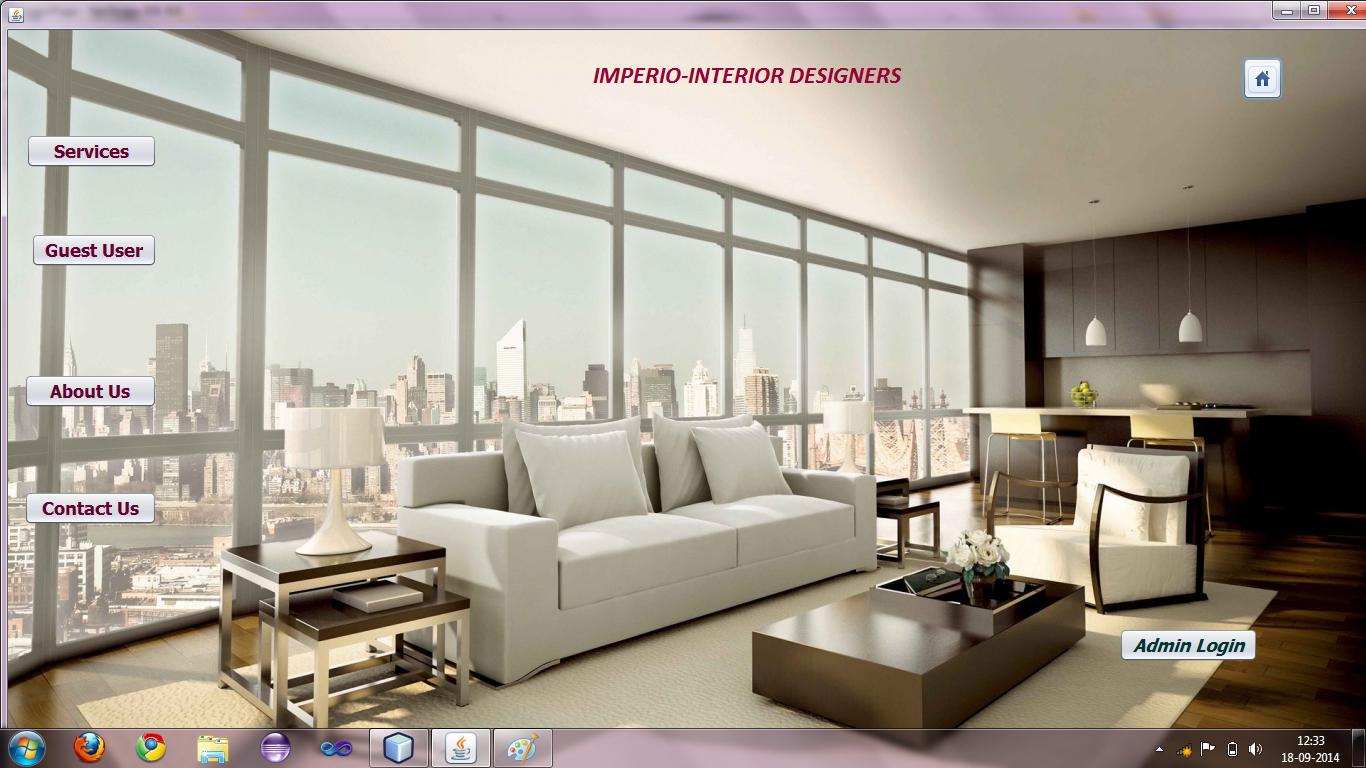
\includegraphics[scale=0.45]{1.png}
\end{center}
\begin{center}
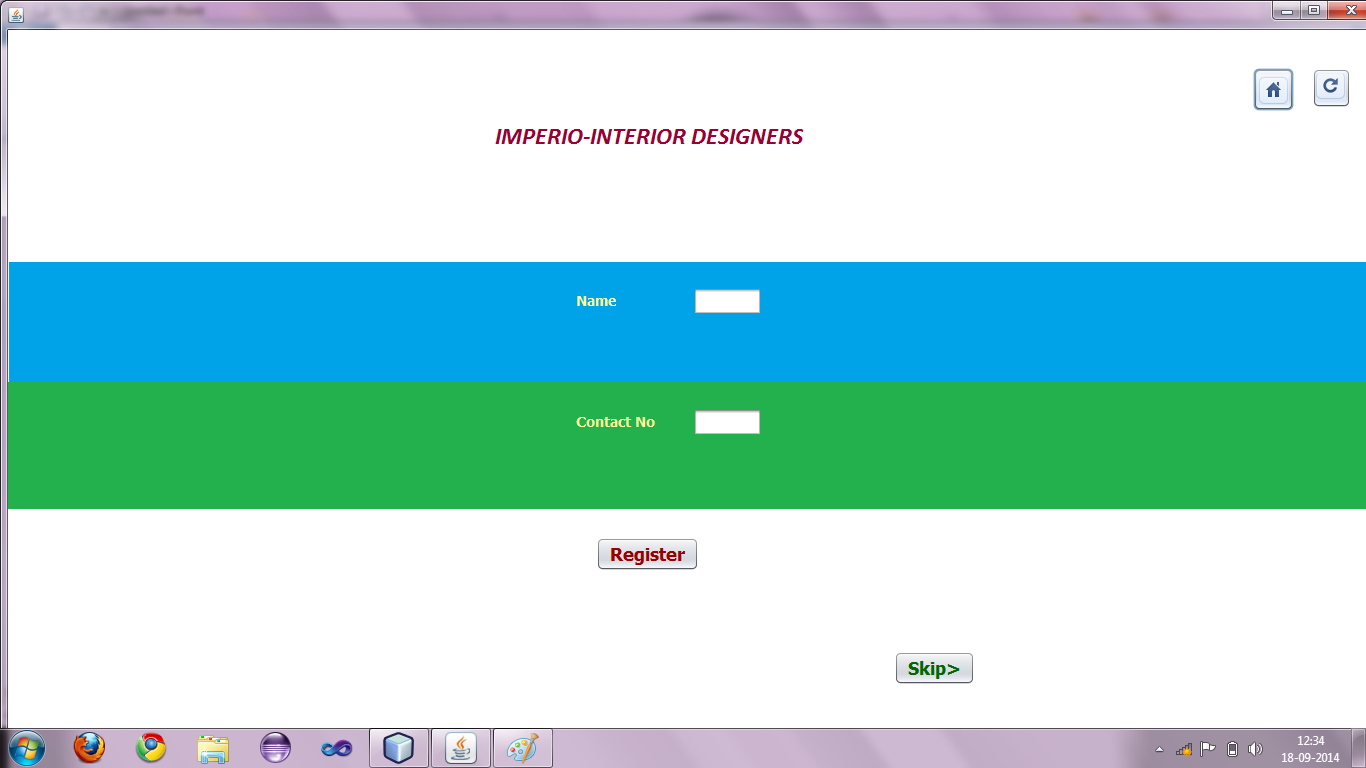
\includegraphics[scale=0.45]{2.png}
\end{center}
\begin{center}
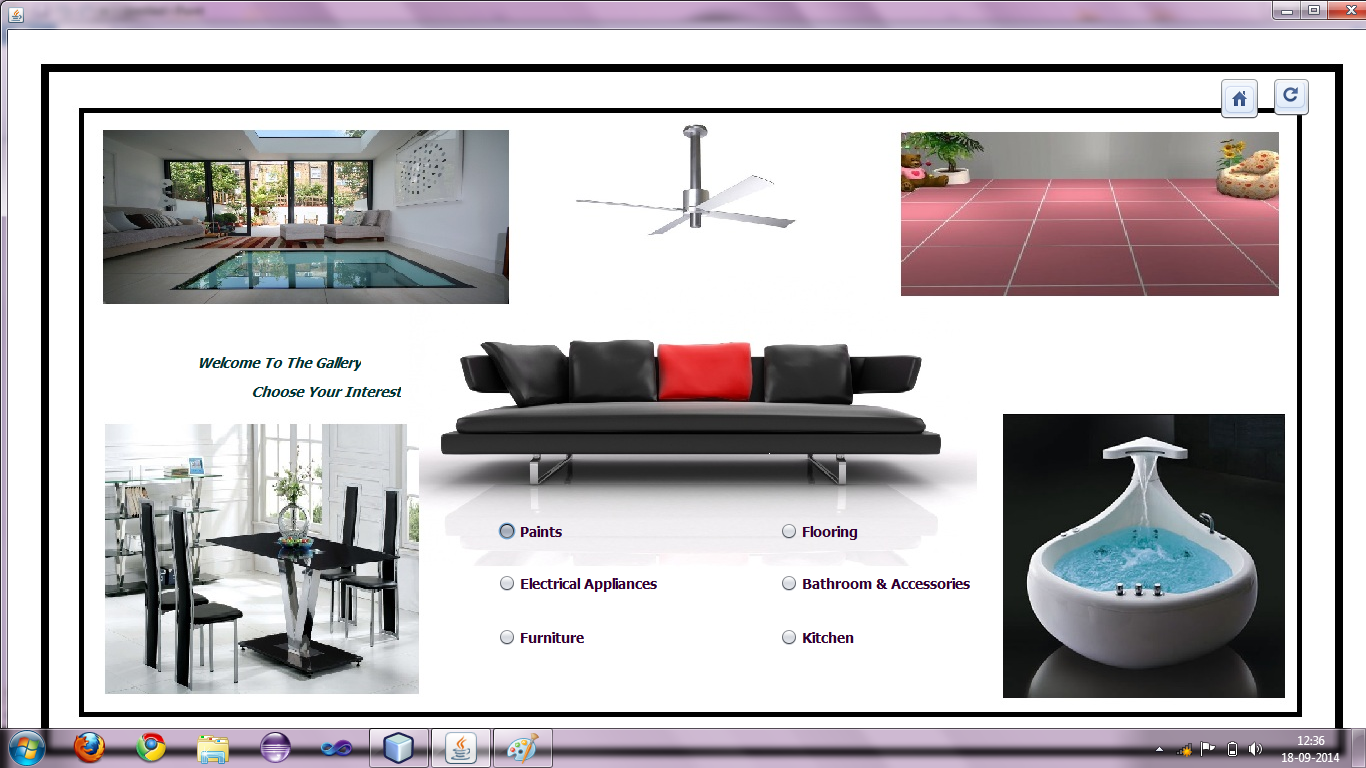
\includegraphics[scale=0.45]{3.png}
\end{center}
\begin{center}
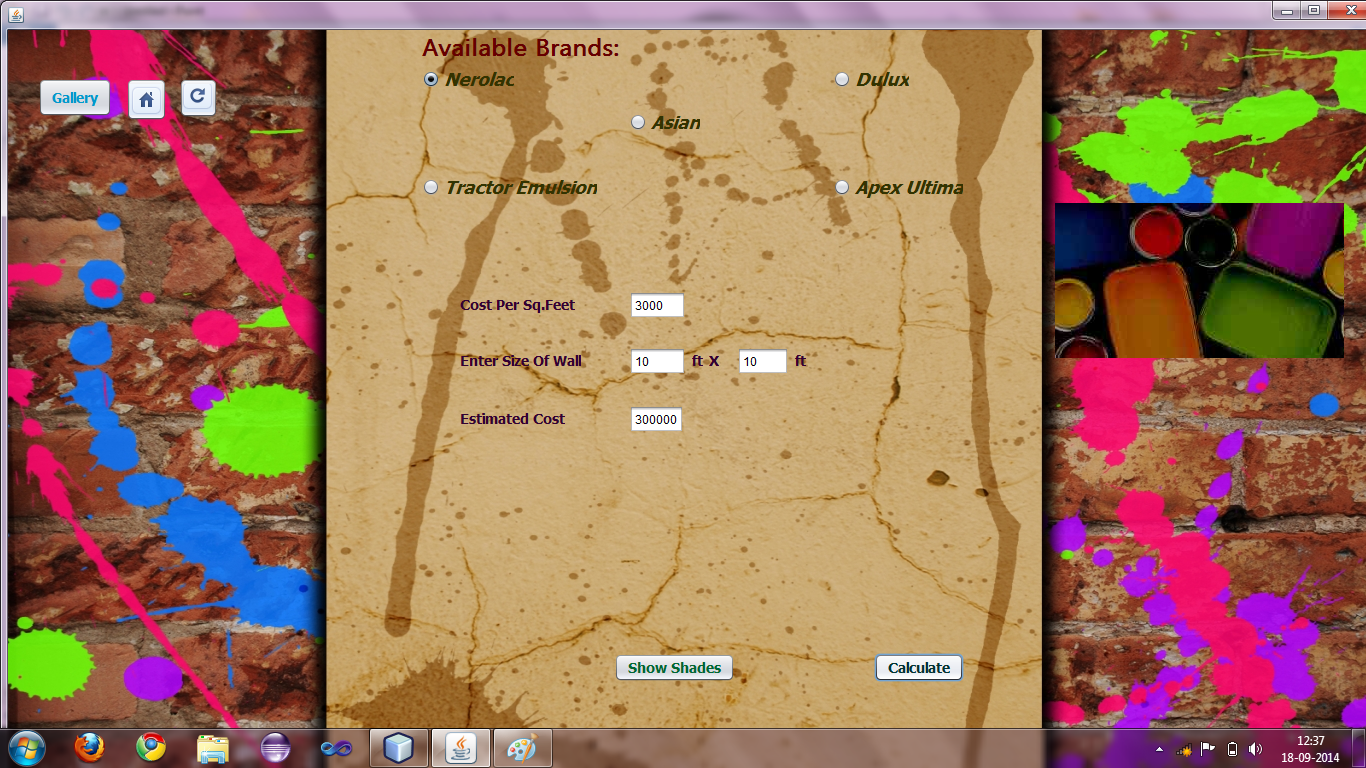
\includegraphics[scale=0.45]{4.png}
\end{center}
\begin{center}
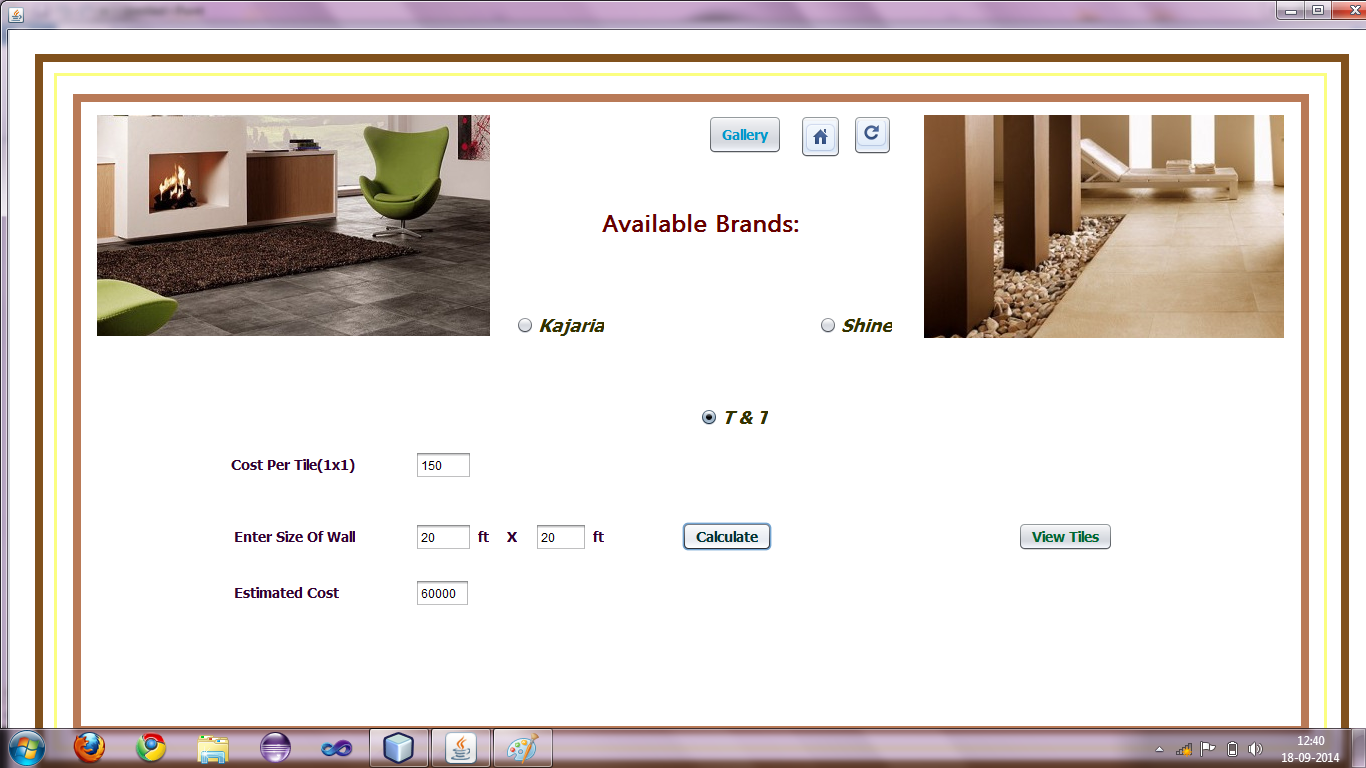
\includegraphics[scale=0.45]{5.png}
\end{center}
\begin{center}
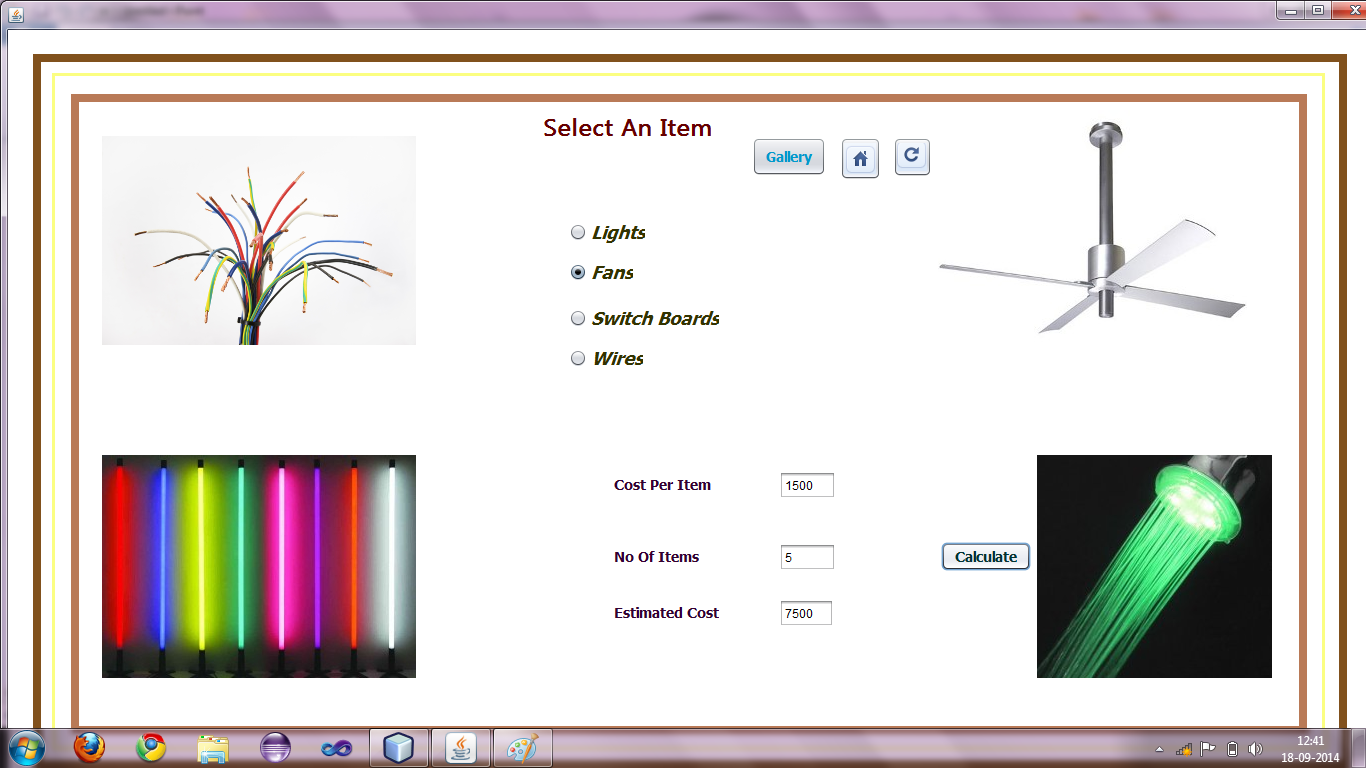
\includegraphics[scale=0.45]{6.png}
\end{center}
\begin{center}
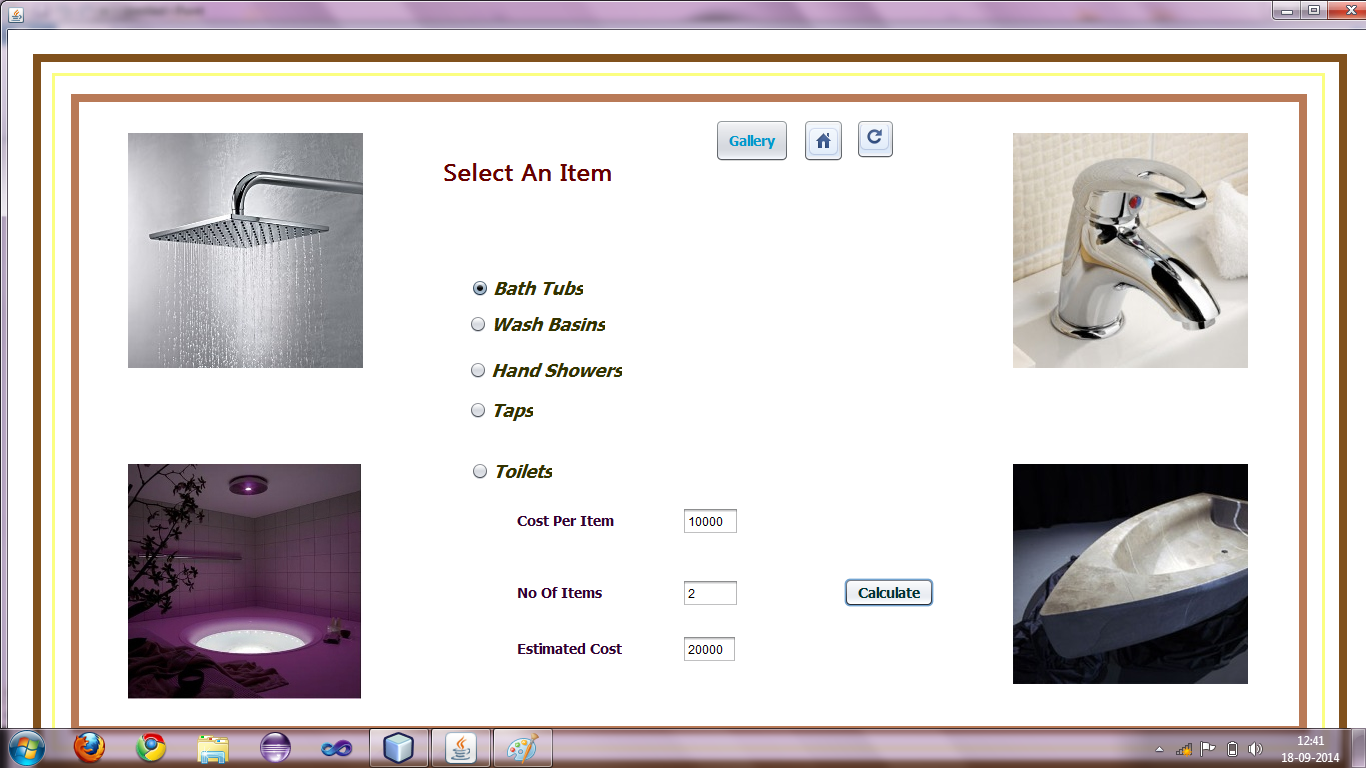
\includegraphics[scale=0.45]{7.png}
\end{center}
\begin{center}
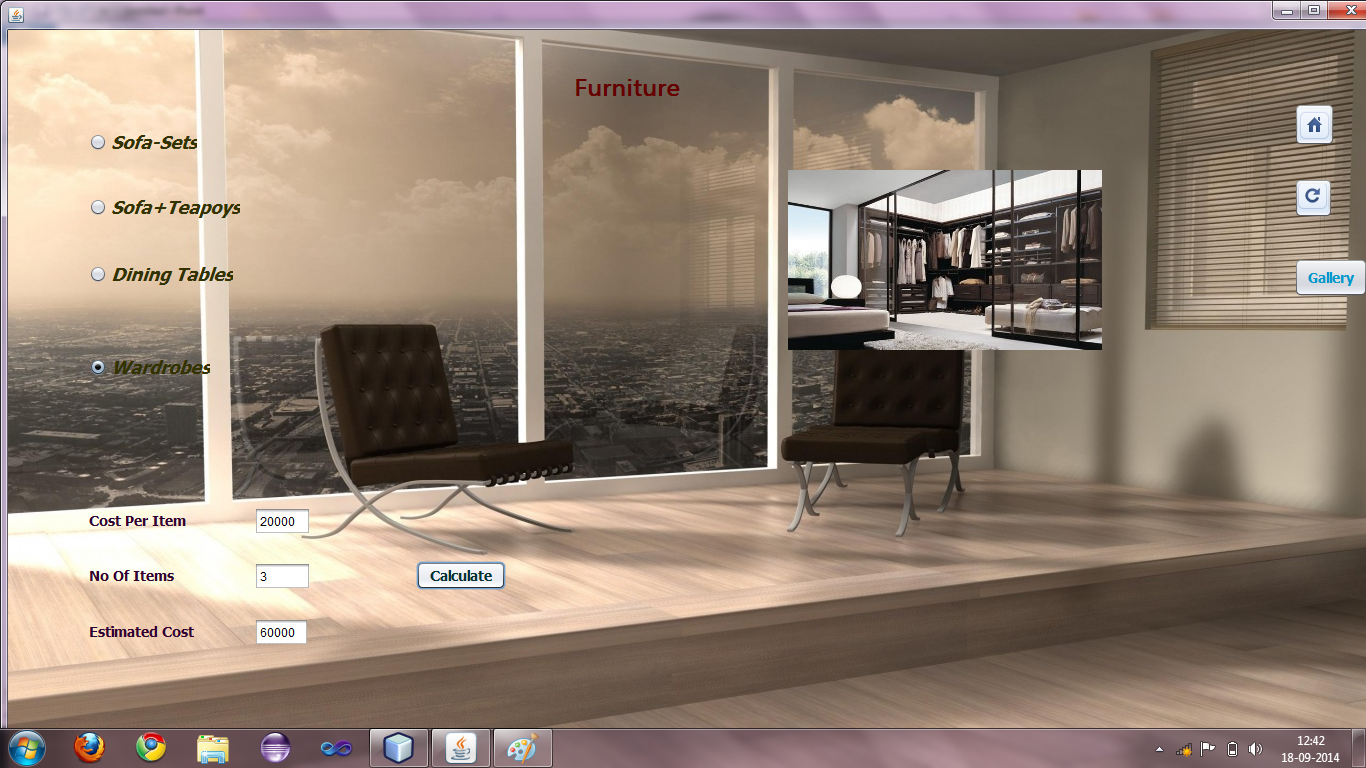
\includegraphics[scale=0.45]{8.png}
\end{center}
\begin{center}
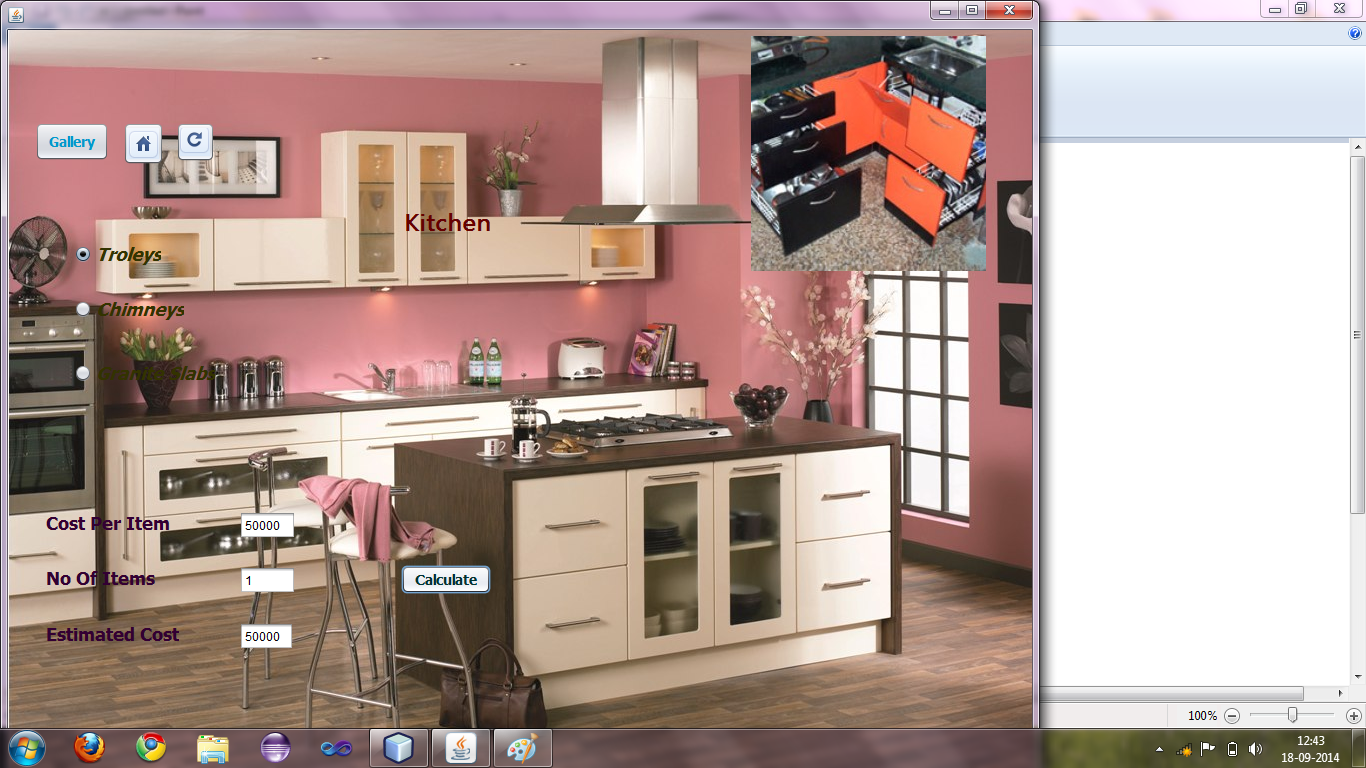
\includegraphics[scale=0.45]{9.png}
\end{center}
\begin{center}
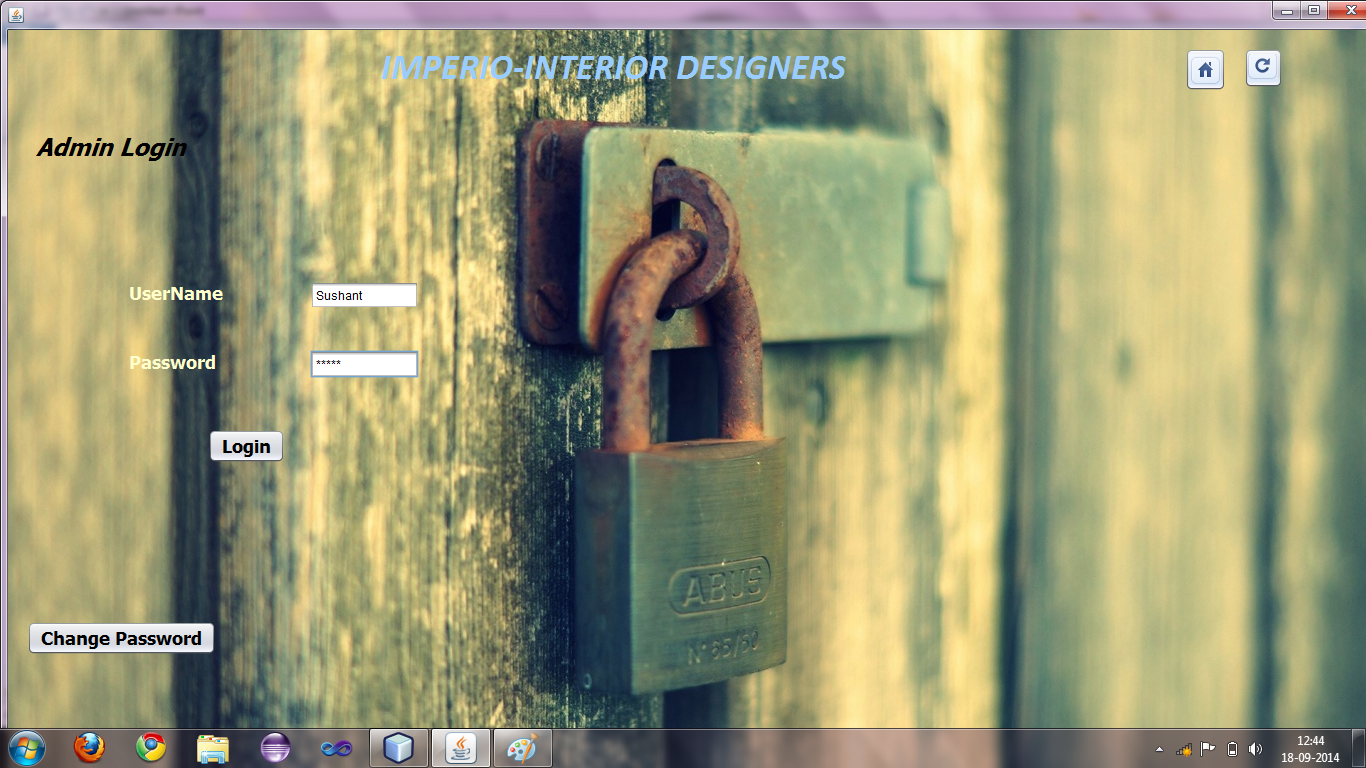
\includegraphics[scale=0.45]{9_1.png}
\end{center}
\begin{center}
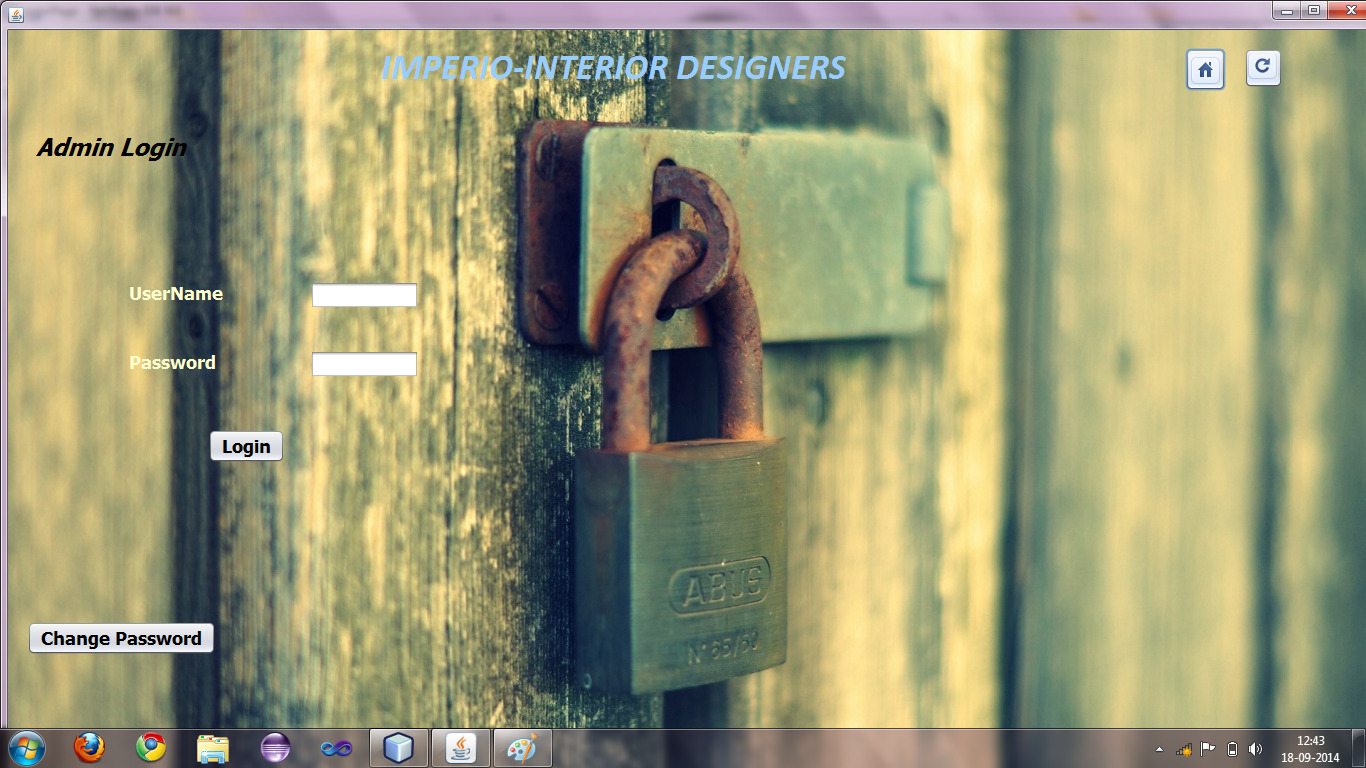
\includegraphics[scale=0.45]{10.png}
\end{center}
\begin{center}
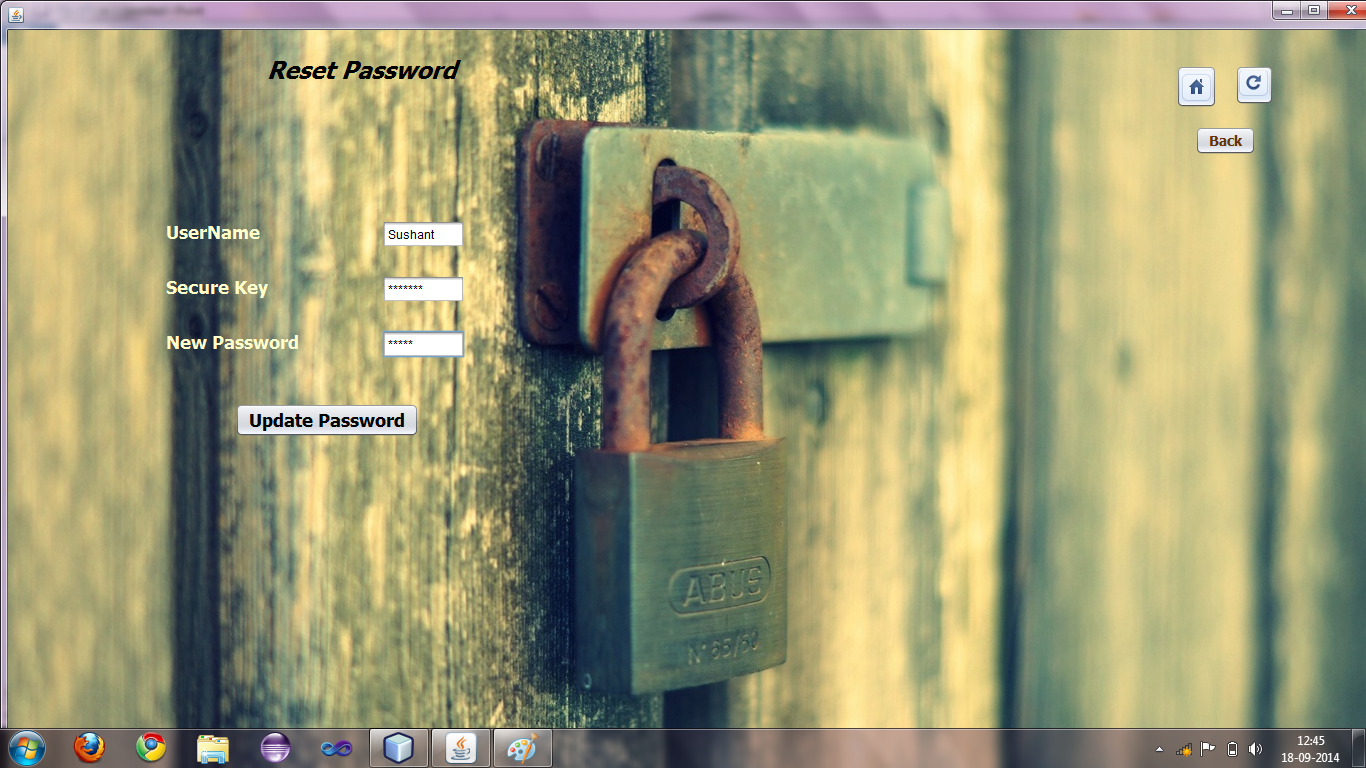
\includegraphics[scale=0.45]{11.png}
\end{center}
\begin{center}
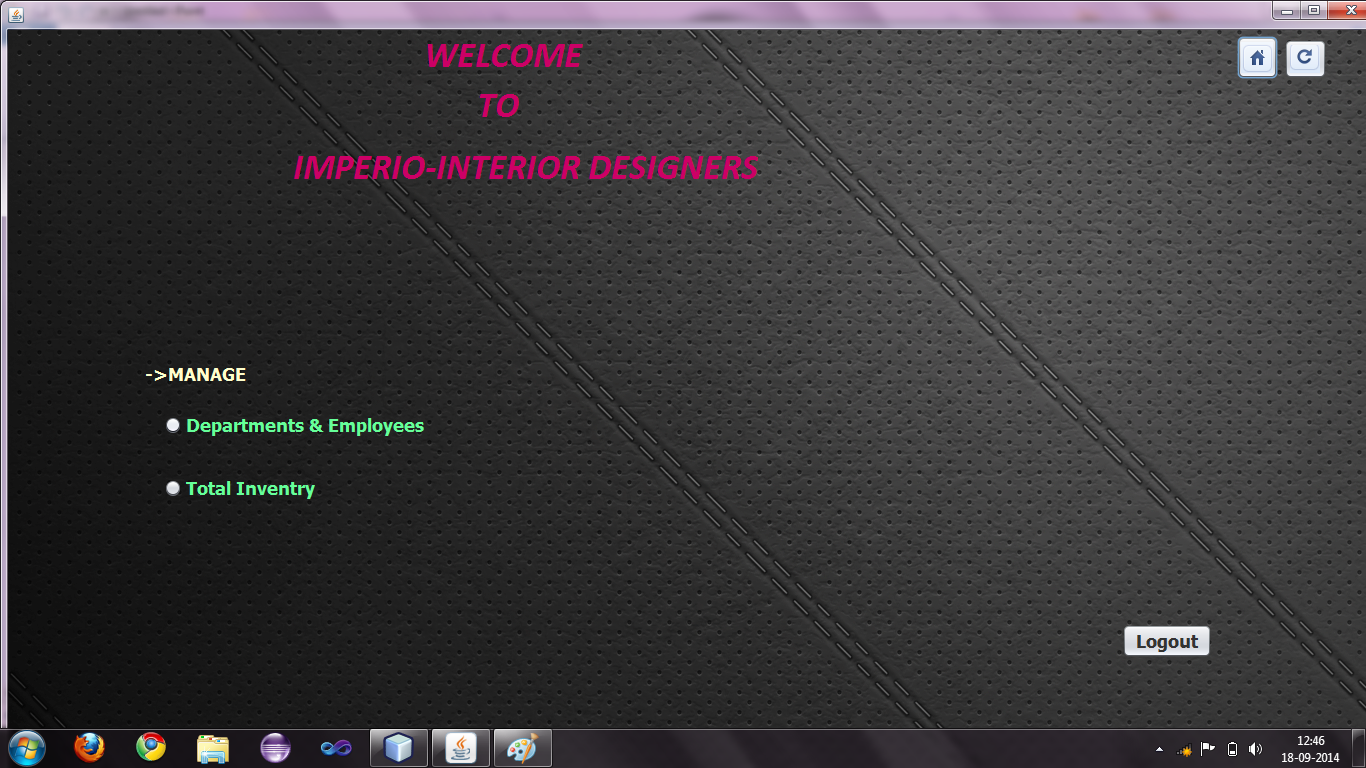
\includegraphics[scale=0.45]{12.png}
\end{center}
\begin{center}
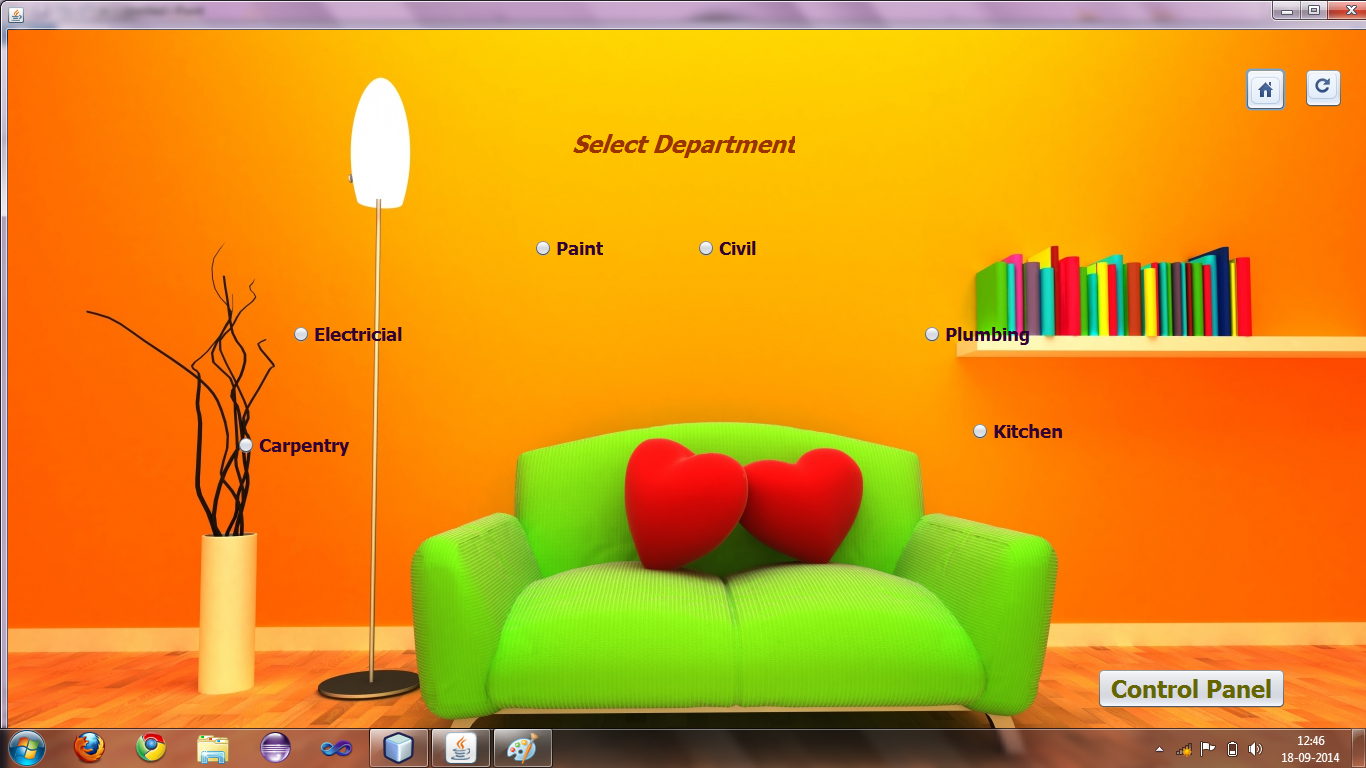
\includegraphics[scale=0.45]{13.png}
\end{center}
\begin{center}
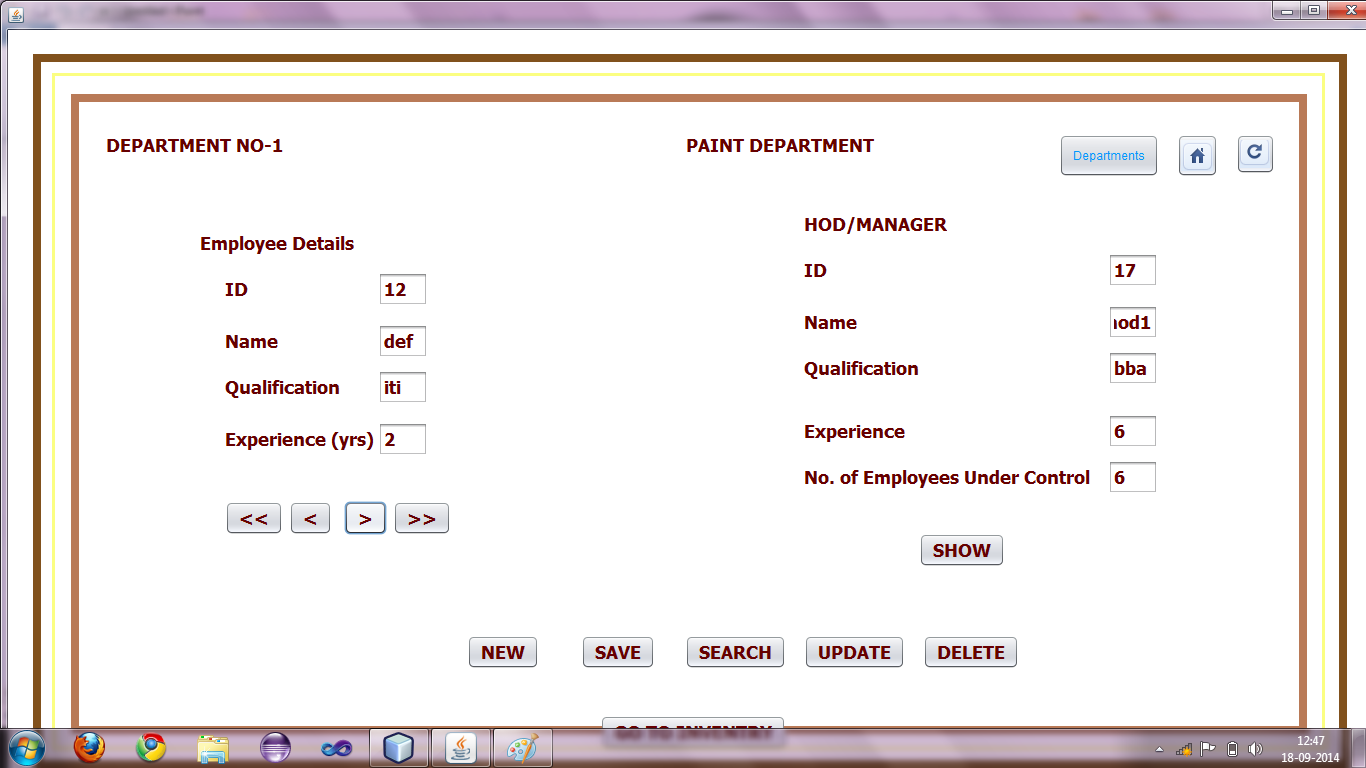
\includegraphics[scale=0.45]{14.png}
\end{center}
\begin{center}
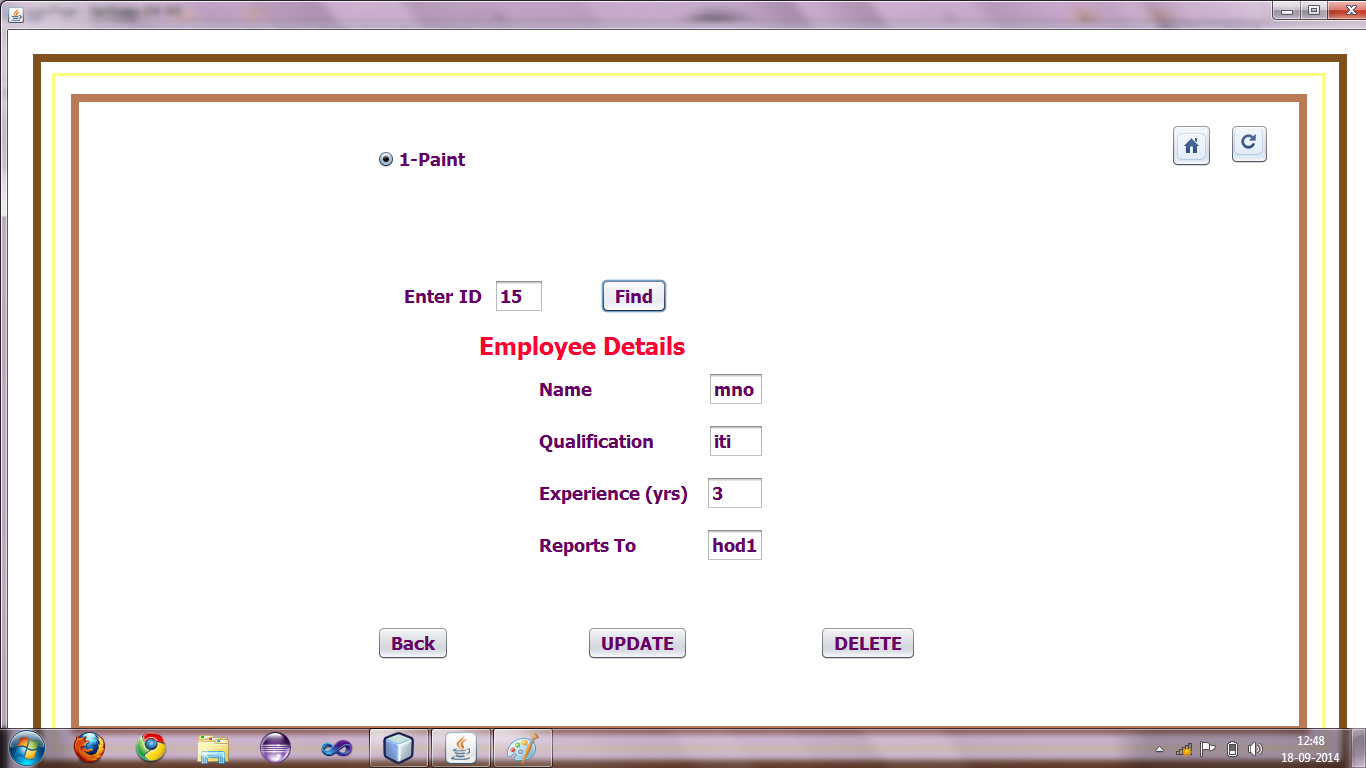
\includegraphics[scale=0.45]{15.png}
\end{center}
\begin{center}
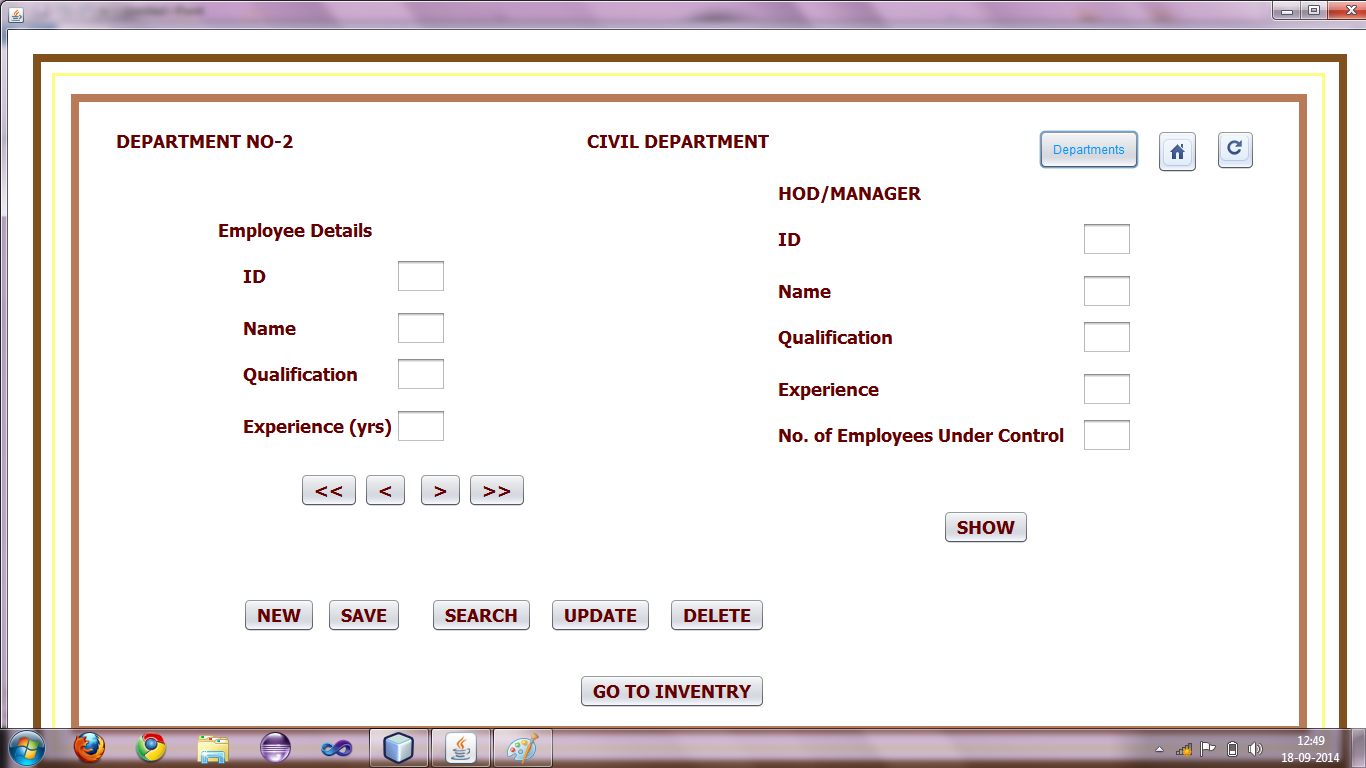
\includegraphics[scale=0.45]{17.png}
\end{center}
\begin{center}
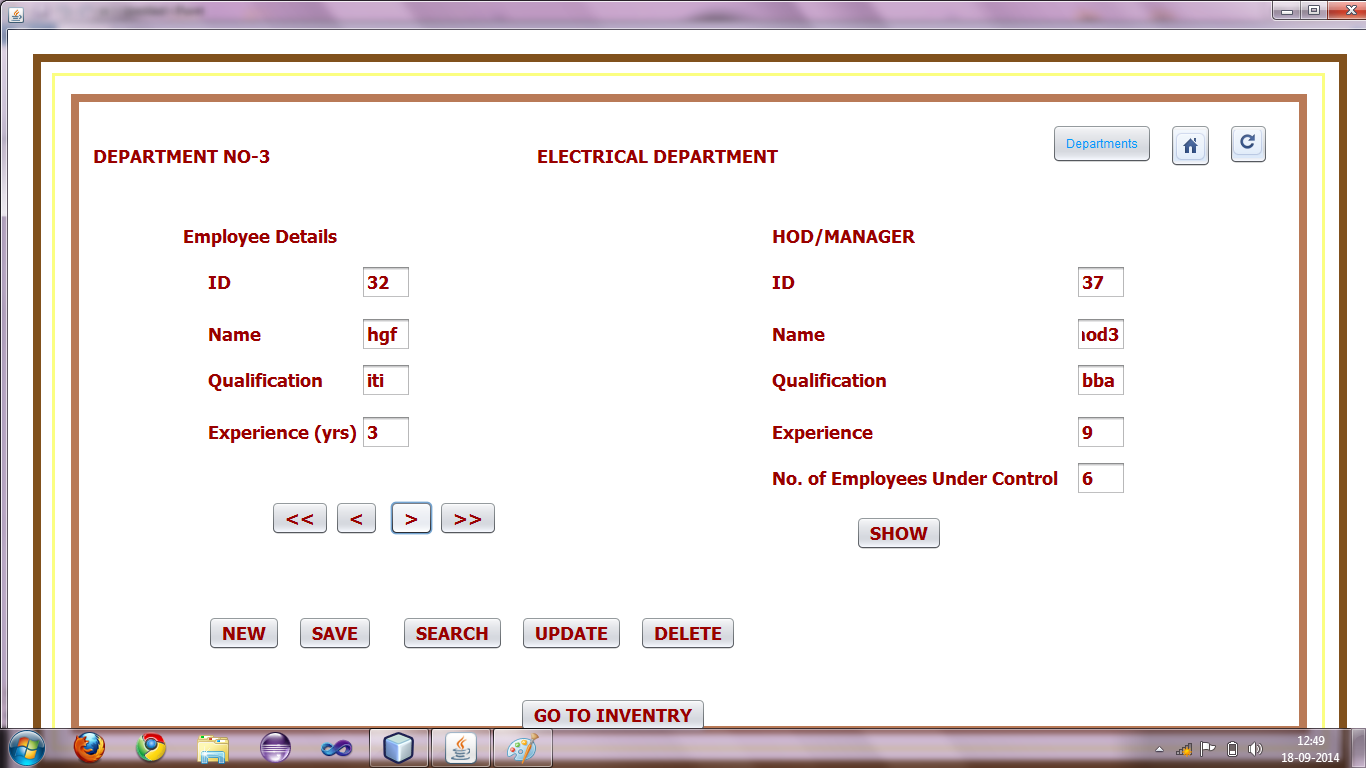
\includegraphics[scale=0.45]{18.png}
\end{center}
\begin{center}
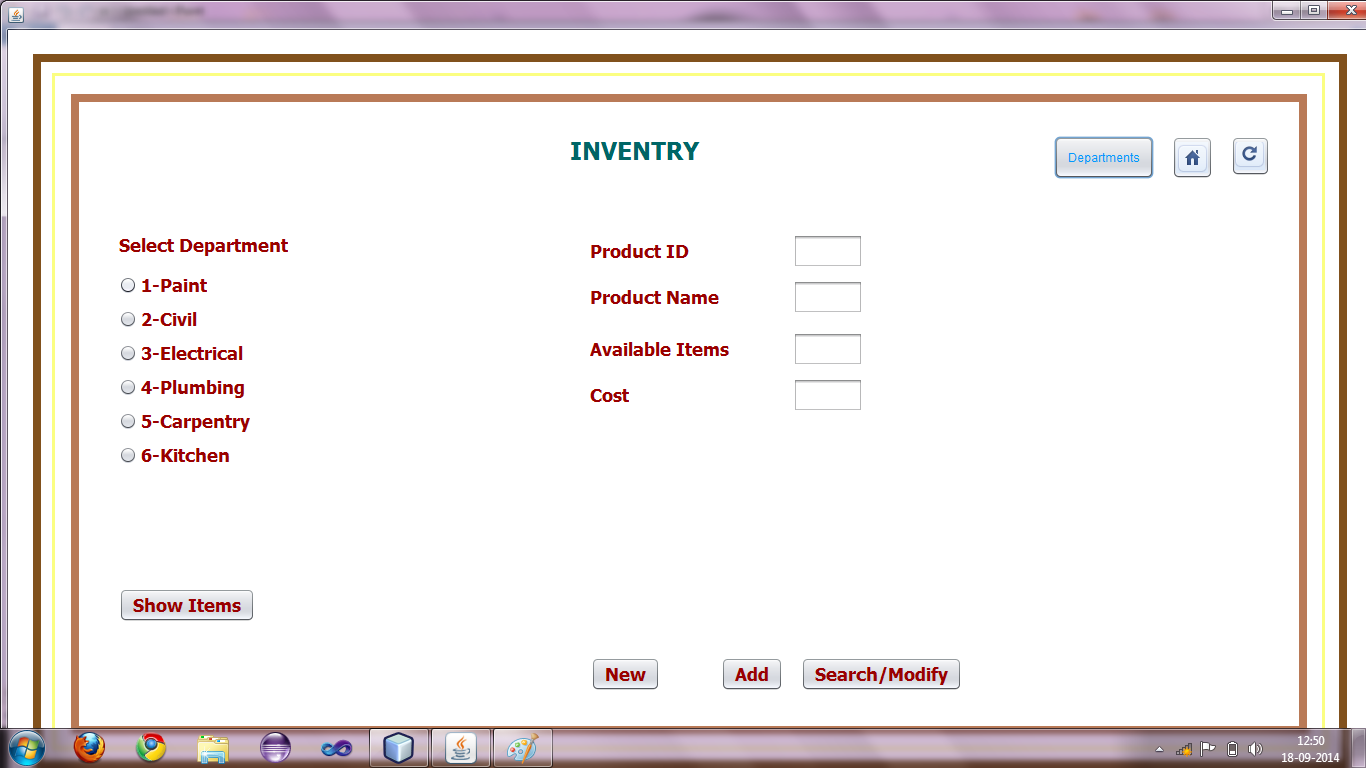
\includegraphics[scale=0.45]{19.png}
\end{center}
\begin{center}
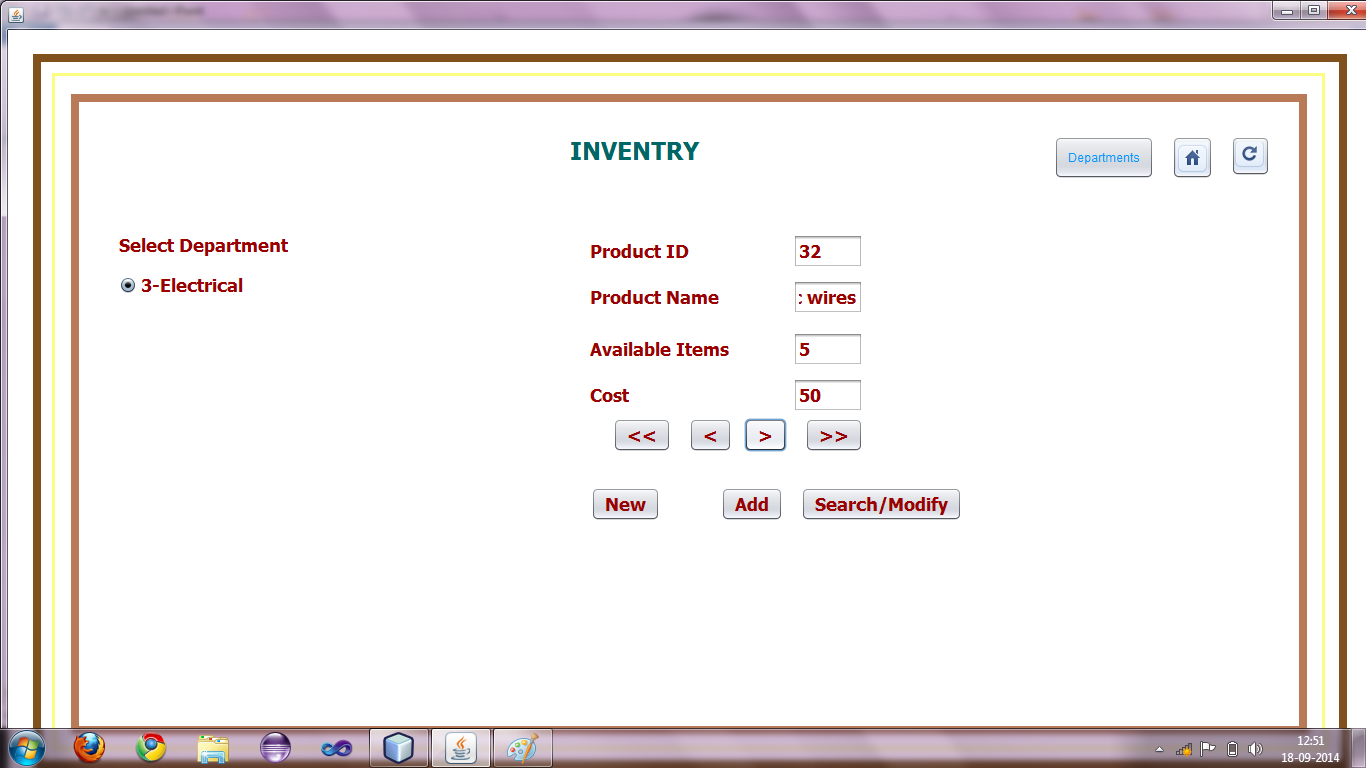
\includegraphics[scale=0.45]{19_1.png}
\end{center}
\begin{center}
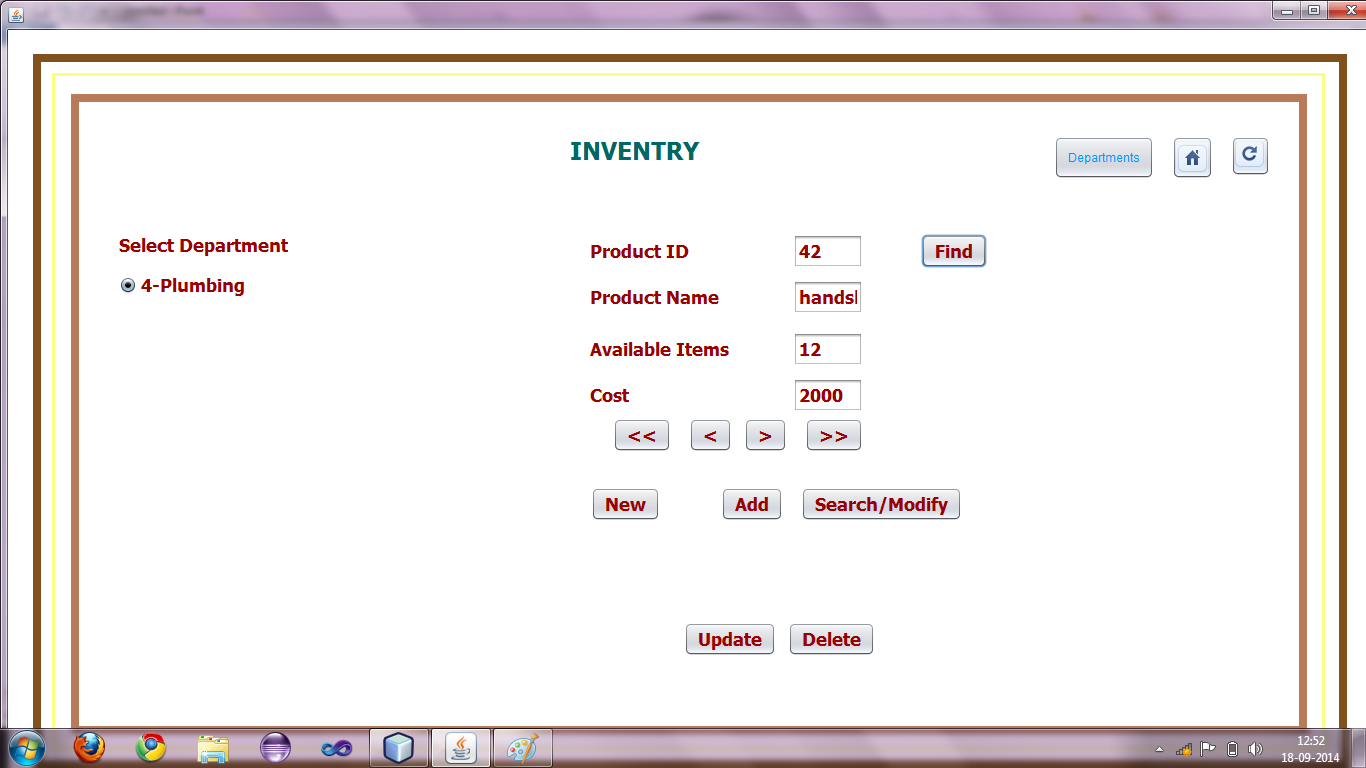
\includegraphics[scale=0.45]{19_2.png}
\end{center}

%END OF CHAPTER7.

\chapter{Acknowledgement.}%Chapter8
The desgining of this database was a challenging task and we are thankful to Professor Kamde for his constant support without which it would have become more difficult to complete this project. Secondly, we would like to indirectly thank the innumerable resources made available to us via the internet, which were available always. Lastly, we'd like to thank all the group members for putting efforts into the project and making it a success.
%END OF CHAPTER8.

\chapter{References.}%Chapter9
[ref MySQL]- \url{www.mysql.com/about/index.html}
\newline[ref NetBeans]- \url{http://netbeans.org/features/platform/}
\newline [ref JDBC] - \url{http://en.wikipedia.org/wiki/Java_Database_Connectivity}
%END OF CHAPTER9.
\end{document}